%Text books : \cite{fraleigh}
%Module 1:
%Introduction to extension fields, algebraic extensions, Geometric Constructions Finite fields.
%(Part VI – Section 29, 31 – 31.1 to 31.18, 32, 33 of the text) (20 hours)
%Module 2:
%Unique factorization domains, Euclidean domains. Gaussian integers and multiplicative norms
%(Part IX – Sections 45,46 & 47 of the text) (20 hours)
%Module 3:
%Automorphism of fields, the isomorphism extension theorem , Splitting fields.
%(Part X – Sections 48 & 49, 50 of the text) (25 hours)
%Module 4:
%Separable extensions, Galois Theory, Illustrations of Galois Theory, Cyclotomic Extensions. (mention the insolvability of the quintic)
%( Sections 51, 53, 54, 55 - 55.1 to 55.6 of the text) (25 hours)

% ME010101 Abstract Algebra
%Module 1 - \cite{fraleigh} 11, 14, 16, 17
%Module 2 - \cite{fraleigh} 34, 36, 37
%Module 3 - \cite{fraleigh} 20, 21, 22, 23
%Module 4 - \cite{fraleigh} 24, 26, 27

%Advanced Abstract Algebra
%Module 1 - \cite{fraleigh} 29, 31, 32, 33
%Module 2 - \cite{fraleigh} 45, 46, 47
%Module 3 - \cite{fraleigh} 48, 49, 50
%Module 4 - \cite{fraleigh} 51, 53, 54, 55

%Missing - \cite{fraleigh} 1, 2, 3, 4, 5, 6, 7, 8, 9, 10,
%	12, 13, 15, 18, 19, 25, 28, 30, 35, 38, 39, 40, 41, 42, 43, 44

%Section 29
\section{Extension Fields \S29}
\subsection*{Previous Results}
\begin{itemize}
	\item Let $R$ be a commutative ring with unity. If $M$ is a maximal ideal in $R$, then $R/M$ is a field. \cite[\S27.9]{fraleigh}
	\item Let $F$ be a field. Every polynomial in $F[x]$ has a unique factorisation into irreducible polynomials except for order and unit.\cite[\S27.27]{fraleigh}
	\item If $\alpha$ is a zero of $f(x) \in F[x]$, then $f(\alpha) = 0$.\cite[\S22.10]{fraleigh}
	\item If $p(x)$ is irreducible over field $F$, then the principal ideal generated by $p(x)$, denoted by $\langle p(x) \rangle$ is a maximal ideal in $F[x]$. \cite[\S27.25]{fraleigh}
	\item Let $R$ be a ring with unity. And $N$ be an ideal of $R$ containing a unit. Then $N = R$.\cite[\S27.5]{fraleigh}
\end{itemize}

\begin{description}
	\item[Basic Goal] Let $F$ be a field and $f(x) \in F[x]$.
	Find a field $E$ such that\\
	$F$ is a subfield of $E$ and there exists a zero of $f(x)$ in $E$ ?
	\item[Extension Field] Let $F$ be a field.
	Field $E$ is an extension field of $F$ if $F$ is a subfield of $E$. \\
	Example : $\mathbb{Q} \le \mathbb{R} \le \mathbb{C}$
	\item[Tower of Fields] A diagrammatic representation emphasising the heirarchy of field extensions in which extension fields appears above their subfields.
\end{description}

\begin{theorem}[Kronecker]
	Let $F$ be field. And $f(x)$ be a non-constant polynomial in $F[x]$. Then there exists an extension field $E$ of $F$ and an $\alpha \in E$ such that $f(\alpha) = 0$.
\end{theorem}
\begin{proof}
	Let $f(x) \in F[x]$. Then $f(x)$ has a unique factorisation into irreducible polynomials in $F[x]$ (except for order and unit). Let $p(x)$ be an irreducible factor of $f(x)$. If $f(x)$ is irreducible over $F$, then $f(x) = cp(x)$. It is enough to construct an extension field $E$ containing both $F$ and $\alpha$ such that ${\color{red}p}(\alpha) = 0$.\\

	If $p(x)$ is irreducible over $F$, then $\langle p(x) \rangle$ is maximal ideal in $F[x]$. Therefore, $F[x]/\langle p(x) \rangle$ is a field, say $E$.\\

	Consider the function $\psi : F \to F[x]/\langle p(x) \rangle$ defined by $\psi(a) = a+\langle p(x) \rangle$. We claim that $\psi : F \to \psi[F]$ is a field isomorphism. $\psi$ is a canonical homomophism with trivial kernel. Thus, $\psi$ is one-to-one.\\

	Let $a,b \in F$. And suppose $\psi(a) = \psi(b)$. It is enough to prove that $a = b$. By the defintion of $\psi$, we have $a+\langle p(x) \rangle = b + \langle p(x) \rangle \implies a-b \in \langle p(x) \rangle$. Suppose $a \ne b$. Then $a-b \ne 0$ and $degree(a-b) = 0$. Then, $\langle p(x) \rangle = F[x]$ which is a contradiction since $\langle p(x) \rangle$ is maximal ideal. Therefore, $\psi$ is one-to-one.\\
	
	We have $p(x)$ is a factor of $f(x)$. Thus $p(\alpha) = 0 \implies f(\alpha) = 0$. Thus, it remains to prove that there exists $\alpha \in F[x]/\langle p(x) \rangle$ such that $p(\alpha) = 0$.\\

	Let $p(x) = a_0 + a_1x + a_2 x^2\cdots + a_n x^n$. Consider $\alpha = x + \langle p(x) \rangle$. Then $p(\alpha) = \phi_\alpha(p)$. Thus, $p(\alpha) = a_0 + a_1(x+\langle p(x) \rangle) + \cdots + a_n(x + \langle p(x) \rangle)^n$. Thus, $p(\alpha) = (a_0+a_1x + a_n x^n) + \langle p(x) \rangle = p(x) + \langle p(x) \rangle = \langle p(x) \rangle = 0$. Therefore, $p(\alpha) = 0$ and $f(\alpha) = 0$.
\end{proof}

\begin{description}
	\item[algebraic over $F$] Let $F \le E$. An element $\alpha \in E$ is algebraic over a field $F$, if there exists $f(x) \in F[x]$ such that $f(\alpha) = 0$.
	\item[transcendental over $F$] Let $F \le E$. An element $\alpha \in E$ is transcendental over the field $F$, if it is not algebraic over $F$.
	\item[algebraic number] We have, $\mathbb{Q} \le \mathbb{C}$. A complex number $\alpha \in \mathbb{C}$ is algebraic if  it is algebraic over $\mathbb{Q}$. Example : $2,\sqrt{2},i$
	\item[transcendental number] A complex number $\alpha \in \mathbb{C}$ is transcendental if it is not an algebraic number. Example : $\pi,e$ (proof excluded)
\end{description}

\textbf{Note 1} : A polynomial $f(x) \in F[x]$ is reducible/irreducible depending upon the choice of the field $F$. For example : $x^2-2$ is irreducible over $\mathbb{Q}$, but is reducible over $\mathbb{R}$.

\textbf{Note 2} : An element $\alpha \in E$ is algebraic/transcendental depending on the choice of the field $F$. For example : $\sqrt{2} \in \mathbb{C}$ is algebraic over $\mathbb{Q}$ since $x^2-2 \in \mathbb{Q}[x]$.

\begin{theorem}
	Let $E$ be an extension field of $F$, and $\alpha \in E$. Let function $\phi_\alpha : F[x] \to E$ be an evaluation homomoprhism. Then $\alpha$ is transcendental  if and only if $\phi_\alpha$ is one-to-one.
\end{theorem}
\begin{proof}
	An element $\alpha \in E$ is transcendental if and only if $f(\alpha) \ne 0$ for any nonzero $f(x) \in F[x]$ where $f(\alpha) = \phi_\alpha(f)$. Thus, kernel of $\phi_\alpha$ is trivial. That is, $\ker(\phi_\alpha) = \{ 0 \}$. Therefore, $\phi_\alpha$ is one-to-one.
\end{proof}

\begin{theorem}
	Let $E$ be an extension field of $F$ and $\alpha \in E$ be algebraic over $F$. Then there exists a unique irreducible polynomial $p(x)$ with minimum degree in $F[x]$ and $p(\alpha) = 0$. If there exists a nonzero polynomial $f(x) \in F[x]$ with $f(\alpha) = 0$, then $p(x)$ divides $f(x)$.
\end{theorem}
\begin{proof}
	Consider evaluation homomorphism $\phi_\alpha : F[x] \to E$ defined by $\phi_\alpha(f) = f(\alpha)$. Then $\ker(\phi)$ is an ideal in $F[x]$. Since every ideal in $F[x]$ is principal, there exists $p(x) \in F[x]$ such that $\langle p(x) \rangle = \ker(\phi)$. And $f(\alpha) = 0 \implies f \in \ker(\phi) = \langle p(x) \rangle$. Thus, $p(x)$ divides $f(x)$.\\

	Suppose $p(x) = r(x)s(x)$. Then $p(\alpha) = r(\alpha)s(\alpha) = 0$. However, $E$ is a field and has no zero divisors. Thus, there exists a polynomial of lesser degree in $\langle p(x) \rangle$ which is a contradiction.
\end{proof}

\begin{description}
	\item[monic polynomial] A polynomial which has $1$ as the coefficient of highest power of $x$. For example : $x^3 - 3x \in \mathbb{Q}[x]$
	\item[$irr(\alpha,F)$] The unique monic, irreducible polynomial $p(x) \in F[x]$ such that $p(\alpha) = 0$. For example, $irr(\sqrt{3},\mathbb{Q}) = x^2-3$
	\item[$deg(\alpha,F)$] The degree of the unique monic, irreducible polynomial $p(x) \in F[x]$ such that $p(\alpha) = 0$. For example, $deg(\sqrt{3},\mathbb{Q}) = 2$.
	\item[simple extension] An extension field $E$ of field $F$ is a simple extension if $E = F(\alpha)$ for some $\alpha \in E$.
\end{description}

\begin{theorem}
	Let $E$ be a simple extension $F(\alpha)$ of field $F$ where $\alpha \in E$ is algebraic over $F$. Let $deg(\alpha,F) = n \ge 1$. Then any element $\beta \in E$ can be uniquely expressed in the form $\beta = b_0 + b_1\alpha + \cdots + b_{n-1}\alpha^{n-1}$ where $b_k \in F$.
\end{theorem}
\begin{proof}
	Consider the evaluation homomorphism $\phi_\alpha : F[x] \to E$ defined by $\phi_\alpha(f) = f(\alpha)$. Then $\phi_\alpha[F[x]] = F(\alpha)$.\\
	
	Let $irr(\alpha,F) = p(x) = x^n + a_{n-1}x^{n-1} + \cdots +a_1x+a_0$. Then, $p(\alpha) = 0$. Thus, 
\begin{equation}
	\alpha^n = -a_{n-1} \alpha^{n-1}-a_{n-2} \alpha^{n-2} - \cdots - a_1\alpha - a_0
\end{equation}
	Clearly, any higher power of $\alpha$ can be eliminated from $f(\alpha)$ as shown below,
	\begin{align*}
		\alpha^{n+1} = & \alpha \alpha^n = -a_{n-1} \alpha^n -a_{n-2} \alpha^{n-1} - \cdots - a_1\alpha^2 - a_0 \alpha \\ 
		 = & a_{n-1} \left( a_{n-1}\alpha^{n-1}+a_{n-2}\alpha^{n-2}+\cdots+a_1\alpha + a_0 \right)\\
		& - a_{n-2}\alpha^{n-1} - a_{n-3}\alpha^{n-2} - a_1\alpha^2 - a_0 \alpha
	\end{align*}

	Thus, in the representation of the element in $F(\alpha)$, the maximum degree of $\alpha$ is $deg(\alpha,F)-1$. Therefore, $\beta \in F(\alpha) \implies \beta = b_0 + b_1\alpha + b_2\alpha^2 + \cdots + b_{n-1}\alpha^{n-1}$.\\

	We can also show that this representation is unique for any $\beta \in F(\alpha)$. Suppose $\beta = b_0'+b_1'\alpha+b_2'\alpha^2+\cdots+b_{n-1}'\alpha^{n-1}$. Then $0 = (b_0 - b_0') + (b_1 - b_1')\alpha + \cdots + (b_{n-1} - b_{n-1}')\alpha^{n-1} = \phi_\alpha(g)$ where $g(x) = (b_0 - b_0') + (b_1 - b_1')x + \cdots + (b_{n-1} - b_{n-1}')x^{n-1}$. Clearly, degree of $g(x)$ is $deg(\alpha,F)-1$ which is less than the minimum degree for a non-zero irreducible polynomial for $\alpha$ over $F$. Thus $g(x) = 0$. In other words, $b_j = b_j',\ \forall j$ and representation for $\beta \in F(\alpha)$ is unique.
\end{proof}
\subsection{Exercises \S29}
%Section 31
\section{Algebraic Extensions \S31}
\begin{description}
	\item[$(G : H)$] is the number of $H$-left cosets in $G$.
	\item[algebraic extension] A extension field $E$ of a field $F$ is algebraic if every element in $E$ is algebraic over $F$.\\
		For example, $\mathbb{C}$ is algebraic over $\mathbb{R}$. But, $\mathbb{R}$ is not algebraic over $\mathbb{Q}$.
	\item[finite extension] A extension field $E$ of field $F$ is a finite extension if $E$ is a finite dimensional vector space over $F$. And $[E:F]$ is the \textbf{dimension of the vector space} $E$ over $F$. Again, $[E:F]$ is the \textbf{degree of the finite extension} $E$ over $F$.\\
		For example, $\mathbb{C}$ is a finite extension of degree $2$ over $\mathbb{R}$, $[\mathbb{C} : \mathbb{R}] = 2$. But, $\mathbb{R}$ is not a finite extension of $\mathbb{Q}$ and $[\mathbb{R} : \mathbb{Q}]$ is infinite.
\end{description}

\begin{theorem}
	Every finite field extensions is an algebraic extension.
\end{theorem}
\begin{proof}
	Let $E$ be a fintie extension of degree $n$ over $F$.Then $[E:F] = n$. Suppose $\alpha \in E$. Clearly, $\{1,\alpha,\alpha^2,\cdots,\alpha^n \}$ is set of $n+1$ vectors from the vector space $E$ over $F$. We know that in a vector space of dimension $n$, any set having $n+1$ vector is linearly dependant. In other words, there exits scalars $c_0,c_1,\cdots,c_n \in F$ (not all zero) such that $c_0+c_1\alpha+c_2\alpha^2+\cdots+c_n\alpha^n = 0$.\\

	Clearly, $f(x) = c_0 + c_1x + c_2x^2 + \cdots +c_nx^n$ is a polynomial in $F[x]$ such that $\phi_\alpha(f) = f(\alpha) = 0$. Since $\alpha \in E$ is arbitrary, every element in $E$ is algebraic over $F$.
\end{proof}

\begin{theorem}
	If $E$ is a finite extension of $F$ and $K$ is a finite extension of $E$. Then $K$ is a finite extension of $F$. And $[K:F] = [K:E][E:F]$.
\end{theorem}
\begin{proof}
	Let $[E:F] = n$ and $[K:E] = m$. Let $\{ \alpha_1,\alpha_2,\cdots,\alpha_n \}$ be basis for vector space $E(F)$ and let $\{ \beta_1,\beta_2,\cdots,\beta_m\}$ be basis for vector space $K(E)$. We claim that $\{\alpha_i\beta_j : 1 \le i \le n,\ 1 \le j \le m \}$ is a basis for the vector space $K(F)$.\\

	Let $\gamma \in K$. Then we have $b_1,b_2,\cdots,b_m \in E$ such that $\gamma = b_1\beta_1+b_2\beta_2+\cdots+b_m\beta_m$. Again, for each $b_j \in E$, we have $a_{ij} \in F$ such that $b_j = a_{1j}\alpha_1+a_{2j}\alpha_2+\cdots+a_{nj}\alpha_n$. Therefore, 
	$$\gamma = \sum_{i=1}^n \sum_{j=1}^m a_{ij} \alpha_i \beta_j$$

	That is, $\{ \alpha_i \beta_j : i =1,2,\cdots,n,\ j=1,2,\cdots,m \}$ spans $K$. It remains to prove that $\{\alpha_i \beta_j \}$ is linearly independent. Suppose it is linearly dependent. Then there exists scalars $c_{i,j} \in F$ (not all zero) such that
	$$\sum_{i=1}^n \sum_{j=1}^m c_{i,j} \alpha_i \beta_j  = \sum_{j=1}^m \left( \sum_{i=1}^n c_{i,j} \alpha_i \right) \beta_j  = 0$$
	
	Let $\sum_{i=1}^n c_{i,j}\alpha_i = b_j$. We know that, $\{ \beta_j : j = 1,2,\cdots,m \}$ is linearly independent. Thus, $\sum_j b_j \beta_j = 0 \implies b_j = 0,\ \forall j$.\\
	
	Again $b_j = 0 \implies \sum_{i = 0}^n c_{i,j}\alpha_i = 0$. Once again, $\{ \alpha_i : i = 1,2,\cdots,n \}$ is linear independent. Thus, $c_{i,j} = 0,\ \forall i,j$. Thus, $\{ \alpha_i \beta_j \}$ is linearly independent. Therefore, $\{ \alpha_i \beta_j \}$ is a basis for the vector space $K(F)$. And $[K : F] = |\{\alpha_i \beta_j : i =1,2,\cdots,n \text{ and } j=1,2,\cdots,m\}|= mn$.
\end{proof}

\begin{corollary}
	Let $F_i$ be fields and $F_{i+1}$ are finite extensions of $F_i$s for $i = 1,2,\cdots,r$. Then $[F_r : F_1] = [F_r : F_{r-1}][F_{r-1}:F_{r-2}]\cdots[F_2:F_1]$.
\end{corollary}
\begin{proof}
	We have, $F_3$ is a finite extension of $F_1$ and 
	\begin{equation}
		[F_3:F_1] = [F_3:F_2][F_2:F_1]
	\end{equation}
	Suppose $F_k$ is a finite extension of $F_1$ and 
	\begin{equation}
		[F_k : F_1] = [F_k:F_{k-1}][F_{k-1}:F_{k-2}] \cdots [F_2:F_1]
	\end{equation}
	\begin{align*}
		[F_{k+1}:F_1] = & [F_{k+1} : F_k][F_k : F_1] \text{ since } F_k \text{ is a finite extension of } F_1\\
		= & [F_{k+1}:F_k][F_k:F_{k-1}][F_{k-1}:F_{k-2}] \cdots [F_2:F_1]
	\end{align*}
\end{proof}

\begin{corollary}
	If $E$ is an extension field of $F$ and $\alpha \in E$ is algebraic over $F$ and $\beta \in F(\alpha)$, then $deg(\beta,F)$ divides $deg(\alpha,F)$.
\end{corollary}
\begin{proof}
	We have, $\deg(\alpha,F) = [F(\alpha) : F]$ and $\deg(\beta,F) = [F(\beta):F]$. Also given that $\beta \in F(\alpha) \implies F(\beta) \le F(\alpha)$. Clearly, $F \le F(\beta) \le F(\alpha)$. Therefore, $[F(\alpha) : F] = [F(\alpha):F(\beta)][F(\beta):F]$. And $[F(\alpha):F(\beta)] = [F(\alpha):F]/[F(\beta):F]$. Clearly, $[F(\beta):F]$ divides $[F(\alpha):F]$.
\end{proof}

\begin{theorem}[algebraic closure]
	Let $E$ be an extension field of $F$. Then $\bar{F}_E = \{ \alpha \in E : \alpha \text{ is algebraic over } E \}$ is a subfield of $E$.
\end{theorem}
\begin{proof}
	Let $\alpha,\beta \in \bar{F}_E$. Then $\alpha,\beta \in E$ are algebraic over $F$. And $F(\alpha,\beta)$ is a finite extension field of $F$. Thus every element in $F(\alpha,\beta)$ are algebraic over $F$. Thus, $\alpha+\beta, \alpha\beta,\alpha-\beta,\alpha/\beta \in \bar{F}_E$. Therefore, $\bar{F}_E$ is a subfield of $E$.
\end{proof}

\begin{corollary}
	The set of all algebraic numbers forms a field.
\end{corollary}
\begin{proof}
	Let $\alpha$ be an algebraic number. Then $\alpha \in \mathbb{C}$ and $\alpha$ is algebraic over $\mathbb{Q}$. Clearly, the set of all algebraic numbers, $\bar{\mathbb{Q}}_\mathbb{C}$ is a subfield of $\mathbb{C}$.
\end{proof}

\begin{description}
	\item[algebraic closure] Let $F$ be a field and $E$ be an extension field of $F$. Then the (smallest) field containing all elements of $E$ which are algebraic over $F$ is the algebraic closure $\bar{F}_E$ of $F$ in $E$.
	\item[algebraically closed] Let $F$ be a field. $F$ is algebraically closed if every non-constant polynomial in $F[x]$ has a zero in $F[x]$.
		
\end{description}

\textbf{Note : } Let $F$ be algebraically closed. Then every irreducible polynomial in $F[x]$ are linear since every non-constant polynomial has a linear factor.

\begin{theorem}
	A field $F$ is algebraically closed if and only if every non-constant polynomial $f(x)$ can be factorised in $F[x]$ into linear factors.
\end{theorem}
\begin{proof}
	Let $F$ be algebraically closed and $f(x)$ be a non-constant polynomial in $F[x]$. Then $f(x)$ has a zero $\alpha \in F$. Then $x-\alpha$ is a factor of $f(x)$. That is, $f(x) = (x-\alpha)g(x)$. If $g(x) \in F[x]$ is non-constant, then it has a zero in $F$. Continuing like this, $f(x)$ can be factorised in $F[x]$ into linear factors.\\

	Suppose every non-constant polynomial in $F[x]$ can be factorised into linear factors. Let $f(x)$ be a non-constant polynomial in $F[x]$. Then $f(x)$ has a linear factor $(ax+b) \in F[x]$. Clearly, $-b/a$ is a zero of $f(x)$.
\end{proof}

\begin{theorem}
	Algebrically closed field has no proper algebraic extensions.
\end{theorem}
\begin{proof}
	Let $E$ be an algebraic extension field of $F$. Then if $\alpha \in E$, we have $irr(\alpha,F) = (x-\alpha)$ since $F$ is algebraically closed, every irreduciblepolynomial in $F[x]$ are linear. Thus $\alpha \in F$. Since $\alpha \in E$ is arbitrary, $F = E$.
\end{proof}

\begin{theorem}[Fundamental Theorem of Algebra]
	$\mathbb{C}$ is algebraically closed.
\end{theorem}
\begin{proof}
	Let $f(z) \in \mathbb{C}[z]$. Suppose $f(z)$ has no zeroes in $\mathbb{C}$. Then $1/f(z)$ is an entire function and as $|z| \to \infty$, $|f(z)| \to \infty$. Thus, $\lim_{|z|\to\infty} \frac{1}{|f(z)|} = 0$. And $1/f(z)$ is bounded.\\
	
	By Liouville's theorem, every bounded entire function is constant. Therefore, $1/f(z)$ is constant and $f(z)$ is also constant. Thus, every non-constant polynomial function in $\mathbb{C}[z]$ has a zero in $\mathbb{C}$.
\end{proof}

\begin{description}
	\item[POSET] Partial Ordered Set - A set together with partial order (reflexive, antisymmetric, transitive relation).\\
		
	For example $(\mathbb{R},<)$, the set of all real numbers together with less than relation is a poset. However, in a poset it is not necessary that two arbitrary elements are comparable. $(\mathbb{C},R)$ defined by $aRb$ if $\Re(a) = \Re(b)$ and $Im(a) < Im(b)$ is a poset in which $2+3i$ and $3+3i$ are not comparable.
	\item[chain] A subset of a poset in which any two elements are comparable. That is, $x,y \in T \implies x < y \text{ OR } y < x$.\\

	For example, For above defined poset $(\mathbb{C},R)$, $T = \{ 2+ib \in \mathbb{C} : b \in \mathbb{R} \}$ is a chain in $\mathbb{C}$.
\end{description}
\begin{lemma}[Zorn]
	If every chain in a poset $S$ has an upper bound. Then $S$ has at least one maximal element in it.
\end{lemma}
\begin{proof}
	Not required ( I think, there is no proof. We just take it as an axiom - always true !. If it is not true for a collection then it is not a set !! )
\end{proof}
\begin{theorem}[Existence of Algebraic Closure]
	Every field $F$ has an algebraic closure $\bar{F}$.
\end{theorem}
\begin{proof}
	Not required (as per syllabus)
\end{proof}

%Section 32
\section{Geometric Constructions}
\begin{description}
	\item[Constructible Number] A real number $\alpha$ is constructible if you can draw a line of length $|\alpha|$, given a line of unit length, in finite steps using straightedge and compass.
\end{description}
\begin{theorem}
	Let $\alpha,\beta$ be constructible real numbers. Then $\alpha + \beta$, $\alpha-\beta$, $\alpha\beta$, $\alpha/\beta$ ($\beta \ne 0$) are also constructible.
\end{theorem}
\begin{proof}
\begin{description}
	\item[$\alpha+\beta$] Draw a line $OA$ of length $|\alpha|$ and extend that line using straight edge $OE$. And draw the line $AB$ of length $|\beta|$ on that extended line, at an point $A$ of the former line extending it. Then $OB$ is a line of length $|\alpha| + |\beta|$.
\begin{center}
\begin{tikzpicture}
	\draw[red] (0,0) -- (5,0);
	\draw (0,0) -- (3,0);
	\draw (0,-0.3) node{$O$};
	\draw (3,-0.3) node{$A$};
	\draw (5,-0.3) node{$B$};
\end{tikzpicture}
\end{center}
	\item[$\alpha-\beta$] Draw a line $OA$ of length $|\alpha|$ and extend that line using straight edge $OE$. And draw the line $AB$ of length $|\beta|$ on that extended line, at an end point $A$ of former line, but in the opposite direction of extension( towards $O$). Then the line $OB$ is of length $|\alpha|-|\beta|$.
\begin{center}
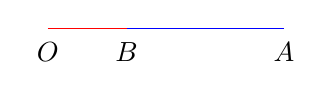
\begin{tikzpicture}
	\draw[blue] (0,0) -- (3,0);
	\draw[red] (0,0) -- (1,0);
	\draw (0,-0.3) node{$O$};
	\draw (3,-0.3) node{$A$};
	\draw (1,-0.3) node{$B$};
\end{tikzpicture}
\end{center}
	\item[$\alpha\beta$] Draw two lines $OA$ and $OB$ of length $|\alpha|$ and $|\beta|$ respectively (with a common end point $O$). Now draw the line of unit length $OP$ along the line $OB$. Construct triangle $OAP$. Draw the line $BQ$ parallel to the line $PA$ through $B$ such that $OQ$ and $OA$ are colinear. Now we have two similar triangles $OPA$ and $OBQ$. Then, the line $OQ$ of length $\| \alpha \beta \|$.
\begin{center}
\begin{tikzpicture}
	\draw[red] (0,0) -- (6,0);
	\draw (0,0) -- (3,0);
	\draw[blue] (0,0) -- (2.5,2);
	\draw (0,0) -- (1.25,1);
	\draw (2.5,2) -- (6,0);
	\draw (1.25,1) -- (3,0);
	\draw (0,-0.3) node{$O$};
	\draw (3,-0.3) node{$A$};
	\draw (1.25,1.3) node{$P$};
	\draw (2.5,2.3) node{$B$};
	\draw (6,-0.3) node{$Q$};
\end{tikzpicture}
\end{center}
	\item[$\alpha/\beta$] Draw two lines $OA$ and $OB$ of length $\| \alpha \|$ and $\| \beta \|$, with a common end point $O$. Draw a line of unit length $OP$ along the line $OB$. Now construct triangle $OBA$. Draw line $PQ$ parallel to $BA$ so that $OQ$ and $OA$ are colinear. Now the triangles $OAB$ and $OQP$ are similar. And the line $OQ$ has length $\| \alpha/\beta \|$.
\begin{center}
\begin{tikzpicture}
	\draw[red] (0,0) -- (6,0);
	\draw (0,0) -- (3,0);
	\draw[blue] (0,0) -- (1.5,2);
	\draw (0,0) -- (0.75,1);
	\draw (1.5,2) -- (6,0);
	\draw (0.75,1) -- (3,0);
	\draw (0,-0.3) node{$O$};
	\draw (3,-0.3) node{$Q$};
	\draw (0.60,1.06) node{$P$};
	\draw (1.5,2.3) node{$B$};
	\draw (6,-0.3) node{$A$};
\end{tikzpicture}
\end{center}
\end{description}
\end{proof}

\begin{corollary}
	The set of all constructible real numbers forms a subfield of the field of real numbers.
\end{corollary}
\begin{proof}
	The set of all constructible real numbers say $H$, contains both $0$ and $1$. since the line of length zero is trivial and line of unit length is provided. And we have, $\forall \alpha,\beta \in H,\ \alpha+\beta,\alpha-\beta,\alpha\beta,\alpha/\beta \in H$. Since $\alpha - \beta \in H$, $0-\beta = -\beta$ which is the additive inverse of $\beta$. And $1/\beta = \beta^{-1}$ is the multiplicative inverse of $\beta$. Thus, the set of all constructible numbers is a subfield of $\mathbb{R}$.
\end{proof}
\textbf{Note : }Since $\mathbb{Q}$ is the prime field of $\mathbb{R}$. Thus, the subfield $H$ of constructible numbers contains $\mathbb{Q}$. That is, all the rational numbers are constructible. And using rational numbers, we can construct all algebraic numbers with help of lines(straight edge) and circles(compass).

\begin{theorem}
 The field of $F$ of constructible numbers consists precisely of all real numbers that we can obtain from $\mathbb{Q}$ by taking square root of positive numbers a finite number of times and applying a finite number of field operations.
\end{theorem}
\begin{proof}

\end{proof}

%Section 33
\section{Finite Fields}

